% !TeX root = ../main.tex
\chapter{Implementation and Deployment}
\label{chap:hien-thuc-trien-khai}

This chapter presents concrete implementation decisions that follow the
design in Chapter~\ref{chap:phan-tich-thiet-ke}: technology versions,
source-code structure, deployment environment configuration, and the
CI/CD process. The goal is to allow a new team member to onboard and
bring up the whole stack on a personal machine or a pilot VPS in under
one hour, while also providing a hardware checklist so the supervising
instructor can estimate the resources required for the pilot phase.

\section{Environment and System Requirements}
\label{sec:environment-requirements}

\subsection{Deployment Environment Tiers}

The system is expected to run in three environment tiers, each with
different hardware requirements and purposes:

\begin{longtable}{|p{2cm}|p{3.2cm}|p{8.3cm}|}
\caption{Three deployment environment tiers.}
\label{tab:envs-c5} \\
\hline
\textbf{Tier} & \textbf{Purpose} & \textbf{Characteristics} \\
\hline
\endfirsthead
\hline
\textbf{Tier} & \textbf{Purpose} & \textbf{Characteristics} \\
\hline
\endhead

\texttt{dev}
    & Local development on team members' machines
    & Docker Compose; uses embedding/STT APIs instead of local models
      to reduce machine load; small dataset; GPU is not required. \\
\hline
\texttt{ci}
    & Automated pipeline on GitHub Actions
    & Testcontainers for PostgreSQL/Redis/Qdrant; mock adapters for
      LLM and STT; sandbox without Internet egress for deterministic
      tests. \\
\hline
\texttt{pilot}
    & Pilot deployment for $\geq 10$ students on a VPS or lab server
    & Public HTTPS domain, Canvas Cloud sandbox; local models can be
      enabled if a GPU is available; daily backup; full OpenTelemetry
      stack. \\
\hline
\end{longtable}

\subsection{Target Operating System}

\textbf{Pilot tier:} \textbf{Ubuntu Server 22.04 LTS} (Jammy
Jellyfish) is the main target OS, selected because:

\begin{itemize}
    \item It is supported by Canonical until April 2027 (5-year LTS)
          and extended with ESM until 2032, long enough for the pilot
          lifecycle and the following production phase of the project.
    \item Updated packages for Docker Engine, Nvidia drivers, and the
          required runtimes are available through official APT sources
          or the official Docker/Nvidia repositories, so no component
          has to be built from source.
    \item It is compatible with \texttt{nvidia-container-toolkit},
          allowing \texttt{video-worker} to access the GPU through
          Docker Compose without manual kernel-module intervention.
\end{itemize}

The backup option \textit{Ubuntu Server 24.04 LTS} (Noble Numbat) is
used if a newer kernel is required, for example with Blackwell-generation
GPU drivers, or if PostgreSQL 18 is needed natively for the built-in
\texttt{uuidv7()} function (on PG 16/17 the system uses the
\texttt{pg\_uuidv7} extension instead).

\textbf{Dev tier:} Linux is not mandatory, so that more team members
can participate. The supported environments are:

\begin{itemize}
    \item \textbf{macOS 14+ (Sonoma) or 15+ (Sequoia):} Docker Desktop
          4.28+; suitable for Apple Silicon (M1/M2/M3) thanks to
          multi-arch images (\texttt{linux/arm64}) for the base images
          in the stack. Local Whisper can run through Metal Performance
          Shaders.
    \item \textbf{Windows 11 + WSL2 (Ubuntu 22.04):} Docker Desktop
          with WSL2 backend; the source code should be mounted inside
          the WSL2 file system to avoid cross-OS I/O latency.
    \item \textbf{Linux Desktop (Ubuntu 22.04/24.04, Fedora 40+):}
          native Docker Engine without a VM, giving the best performance
          for developers with a GPU.
\end{itemize}

\textbf{CI tier:} the default GitHub Actions runner
\texttt{ubuntu-22.04} is used, with a planned move to
\texttt{ubuntu-24.04} after April 2025 when GitHub changes its default.

\subsection{Hardware Requirements by Tier}
\label{subsec:hardware-tiers}

Table~\ref{tab:hardware-tiers} lists the minimum and recommended
configurations for each environment tier. It is used as a checklist
when purchasing machines or renting VPS resources.

\begin{longtable}{|p{2.8cm}|p{1.6cm}|p{1.6cm}|p{2cm}|p{1.7cm}|p{2.7cm}|}
\caption{Hardware requirements by environment tier.}
\label{tab:hardware-tiers} \\
\hline
\textbf{Tier} & \textbf{CPU} & \textbf{RAM} & \textbf{Disk} & \textbf{GPU}
    & \textbf{Notes} \\
\hline
\endfirsthead
\hline
\textbf{Tier} & \textbf{CPU} & \textbf{RAM} & \textbf{Disk} & \textbf{GPU}
    & \textbf{Notes} \\
\hline
\endhead

Minimum dev & 4 cores (i5 gen 10+/\allowbreak Ryzen 5/Apple M1) & 16GB & 50GB SSD
    & Optional & Use APIs for embedding/STT instead of local models. \\
\hline
Recommended dev & 8 cores & 32GB & 100GB SSD & Optional 4GB VRAM
    & Can run Whisper small and BGE-M3 locally. \\
\hline
CI runner & 2 cores & 8GB & 30GB & No
    & GitHub Actions \texttt{ubuntu-22.04} or self-hosted. \\
\hline
Minimum pilot & 4 cores & 16GB & 100GB SSD & No
    & Enough for 10--20 concurrent students when using STT/\allowbreak embedding APIs. \\
\hline
Recommended pilot & 8 cores & 32GB & 200GB NVMe & 1x 8GB VRAM GPU
    (for example RTX 3060/\allowbreak 4060 or NVIDIA T4)
    & Can run Whisper medium + BGE-M3 locally; Gemini API is still
      required. \\
\hline
Reference production & 16 cores+ & 64GB+ & 500GB NVMe + separate backup
    & 2x 16GB+ VRAM GPUs (for example L4 or A10)
    & Move PostgreSQL/\allowbreak Qdrant to managed services; many
      courses/classes in parallel. \\
\hline
\end{longtable}

\textbf{Reason for choosing 8GB VRAM for the pilot:} Whisper
\texttt{medium} (769M parameters) requires approximately 5GB VRAM
during inference, while \texttt{small} (244M parameters) requires
approximately 2GB; BGE-M3 dense embedding requires another
approximately 2GB when loaded in FP16. With 8GB VRAM, Whisper medium
and BGE-M3 can run at the same time without unloading and reloading
models between requests.

\subsection{RAM Allocation per Container}
\label{subsec:ram-allocation}

Table~\ref{tab:ram-allocation} describes the expected RAM allocation
for each service in the Docker Compose stack. The minimum dev load is
around 10GB, while the pilot load is around 20GB, excluding Docker
daemon overhead ($\approx$ 500MB) and the host OS ($\approx$ 1--2GB).

\begin{longtable}{|p{3.7cm}|p{1.5cm}|p{1.8cm}|p{6cm}|}
\caption{Expected RAM allocation for each service.}
\label{tab:ram-allocation} \\
\hline
\textbf{Service} & \textbf{Dev} & \textbf{Pilot} & \textbf{Configuration notes} \\
\hline
\endfirsthead
\hline
\textbf{Service} & \textbf{Dev} & \textbf{Pilot} & \textbf{Configuration notes} \\
\hline
\endhead

PostgreSQL 16/17 & 512MB & 2GB
    & \texttt{shared\_buffers} 25\% of container RAM,
      \texttt{work\_mem} 16MB, \texttt{effective\_cache\_size} 50\%. \\
\hline
Redis 7 & 256MB & 1GB
    & AOF persistence; stores BullMQ queues and LTI sessions. \\
\hline
Qdrant 1.10+ & 512MB & 2GB
    & Int8 quantization for dense vectors (4x smaller footprint);
      \texttt{available\_on\_ram=true} for the hot collection. \\
\hline
Neo4j 5 Community & 1GB & 2GB
    & Heap 50\%, page cache 50\%; \textit{property-based multi-tenancy},
      not multi-instance. \\
\hline
MinIO & 256MB & 512MB & Small cache; data persists on disk. \\
\hline
\texttt{web-bff} (Next.js 14) & 256MB & 512MB
    & SSR + LTI routes; node --max-old-space-size=384. \\
\hline
\texttt{core-api} (NestJS 10) & 512MB & 1GB
    & DB connection pool 20, Outbox poller daemon. \\
\hline
\texttt{chat-service} (FastAPI) & 512MB & 1GB
    & Uvicorn 2 workers, SSE streaming; concurrency 50/worker. \\
\hline
\texttt{document-worker} & 3GB & 4GB
    & \textbf{BGE-M3 model $\approx$ 2GB} (FP16) plus parser/PDF buffer
      1GB. \\
\hline
\texttt{enrichment-worker} & 512MB & 1GB
    & I/O-bound, calls LLM APIs; does not load a model. \\
\hline
\texttt{video-worker} (Go) & 2GB & 4GB
    & \textbf{Whisper model 1--1.5GB} plus FFmpeg subprocess buffer. \\
\hline
Prometheus & 256MB & 1GB & Scrape interval 15s; 7-day retention. \\
\hline
Grafana & 256MB & 512MB & UI only; does not store data. \\
\hline
Loki & 256MB & 1GB & Log aggregation with compactor. \\
\hline
Tempo & 256MB & 1GB & Trace storage; 10\% sampling. \\
\hline
Caddy & 64MB & 128MB & Reverse proxy + Let's Encrypt ACME. \\
\hline
\textbf{Total} & \textbf{$\approx$10GB} & \textbf{$\approx$20GB}
    & Excludes Docker daemon and host OS overhead. \\
\hline
\end{longtable}

\textbf{Scaling note:} If the pilot expands to $\geq 50$ concurrent
students, Qdrant RAM should be increased to 4GB and PostgreSQL to 4GB;
\texttt{chat-service} should scale to 3 replicas with 1GB per replica.
When total load exceeds 32GB, PostgreSQL and Qdrant should be moved to
managed services or separate nodes.

\subsection{Pinned Technology Versions}
\label{subsec:tech-versions}

Table~\ref{tab:tech-versions} lists the pinned versions of runtime and
infrastructure components in the pilot stack. Versions are selected by
three criteria: (i) generally available for at least 6 months, (ii)
supported by an active community, and (iii) compatible with Ubuntu
22.04 LTS through official repositories (APT or official Docker Hub).

\begin{longtable}{|p{4.3cm}|p{3.7cm}|p{5.5cm}|}
\caption{Pinned technology versions for the pilot tier.}
\label{tab:tech-versions} \\
\hline
\textbf{Component} & \textbf{Version} & \textbf{Notes} \\
\hline
\endfirsthead
\hline
\textbf{Component} & \textbf{Version} & \textbf{Notes} \\
\hline
\endhead

Host OS & Ubuntu Server 22.04 LTS & HWE 6.x kernel if a newer GPU is
    required. \\
\hline
Docker Engine & 25.0+ & API 1.44, BuildKit enabled by default. \\
\hline
Docker Compose & v2.24+ & Supports \texttt{deploy.resources} for
    non-swarm deployments. \\
\hline
\texttt{nvidia-container-}\allowbreak\texttt{toolkit} & 1.15+ & GPU passthrough for
    \texttt{video-worker}. \\
\hline
Node.js & 20 LTS (Iron) & \texttt{web-bff} + \texttt{core-api}. \\
\hline
Next.js & 14.2+ & App Router + Server Actions + Streaming SSE. \\
\hline
NestJS & 10.3+ & Fastify adapter; module per bounded context. \\
\hline
Python & 3.11 & \texttt{document-worker}, \texttt{enrichment-worker},
    \texttt{chat-service}. \\
\hline
FastAPI & 0.110+ & Native SSE streaming through
    \texttt{StreamingResponse}. \\
\hline
Go & 1.22+ & \texttt{video-worker}; uses \texttt{goroutine} for the
    FFmpeg pipeline. \\
\hline
PostgreSQL & 18 recommended & Native \texttt{uuidv7()} from 18;
    on PG 16/17, install the \texttt{pg\_uuidv7} extension. \\
\hline
Redis & 7.2 & Streams + Pub/Sub for BullMQ. \\
\hline
Qdrant & 1.10+ & Hybrid search (dense + sparse) + payload index. \\
\hline
Neo4j & 5.x Community & Range Index for property-based multi-tenancy. \\
\hline
MinIO & RELEASE.2024-Q3+ & S3 API compatibility, presigned URLs. \\
\hline
BullMQ & 5.x & Queue + Worker + Sandbox processor. \\
\hline
BGE-M3 (embedding) & v1.0 & Multilingual + sparse + dense + ColBERT. \\
\hline
Whisper & \texttt{small}/\allowbreak\texttt{medium}/\allowbreak\texttt{large-v3} & Depends
    on VRAM; fallback to OpenAI Whisper API. \\
\hline
Gemini API & \texttt{gemini-1.5-pro},
    \texttt{gemini-1.5-flash} & Pro for cards/quizzes, Flash for
    curriculum extraction. \\
\hline
Caddy & 2.7+ & Reverse proxy + automatic ACME. \\
\hline
Prometheus / Grafana / Loki / Tempo
    & v2.x / v11.x / v3.x / v2.x & OpenTelemetry stack. \\
\hline
\end{longtable}

\subsection{Network and Domain Requirements}
\label{subsec:network-req}

\begin{itemize}
    \item \textbf{Inbound:} public 443/tcp for LTI launches from Canvas
          and for instructor/student access. Port 80 only redirects
          301 to HTTPS and does not serve real traffic.
    \item \textbf{Outbound:} 443/tcp to Canvas (LTI AGS callback,
          JWKS), Gemini API
          (\texttt{generativelanguage.googleapis.com}), and the fallback
          STT provider (OpenAI/AssemblyAI if configured).
    \item \textbf{Internal Docker network:} \texttt{ai\_internal}
          bridge, with \textit{no database container ports exposed to
          the host} in production. Only \texttt{caddy} binds to the
          host network.
    \item \textbf{Domain name:} one subdomain with a valid SSL
          certificate (Let's Encrypt through Caddy automatically), for
          example \texttt{lvtn-ai.example.edu.vn}. Canvas only accepts
          an LTI Tool with valid HTTPS; a self-signed certificate cannot
          be used.
\end{itemize}

% \section{Source Code Structure}
% \label{sec:code-structure}

% \subsection{Monorepo Organization}

% The source code is organized as a monorepo with a pnpm workspace for
% TypeScript and a Poetry workspace for Python. They live in the same
% repository to make cross-language refactoring easier when gRPC contracts
% or event schemas change:

% \begin{verbatim}
% lvtn-ai/
% |-- apps/
% |   |-- web-bff/                # Next.js 14, App Router
% |   |-- core-api/               # NestJS, business logic
% |   |-- chat-service/           # FastAPI, RAG + SSE
% |   |-- document-worker/        # Python + BullMQ
% |   |-- enrichment-worker/      # Python + BullMQ
% |   `-- video-worker/           # Go + FFmpeg + Whisper
% |-- packages/
% |   |-- shared-contracts/       # Protobuf, OpenAPI, Zod schema
% |   |-- shared-domain-py/       # Python: Hexagonal Port (ABC)
% |   |-- shared-domain-ts/       # TypeScript: domain entity, DTO
% |   `-- shared-eslint-config/
% |-- infra/
% |   |-- docker-compose.yml      # Pilot stack
% |   |-- docker-compose.dev.yml  # Dev override
% |   |-- caddy/Caddyfile
% |   |-- prometheus/prometheus.yml
% |   |-- grafana/dashboards/
% |   |-- postgres/migrations/    # Atlas or Liquibase
% |   `-- neo4j/cypher-init/
% |-- tools/
% |   |-- seed-data/
% |   |-- eval-retrieval/         # Recall@K, MRR script
% |   `-- benchmark/
% |-- docs/
% |   |-- ARCHITECTURE.md
% |   |-- RUNBOOK.md
% |   `-- ONBOARDING.md
% |-- .github/workflows/          # CI/CD pipeline
% |-- pnpm-workspace.yaml
% |-- pyproject.toml              # Root Poetry
% `-- README.md
% \end{verbatim}

% The reason for choosing a monorepo instead of polyrepo is that the
% contracts between runtimes (BullMQ event schemas, gRPC proto files, JWT
% claim shapes) often change at the same time as their implementations.
% If the project were split into multiple repositories, each schema change
% would require pull requests in several places and cross-version locking.
% With a monorepo, one pull request can update both producer and consumer
% of the same event, and CI can run global integration tests.

% \subsection{Hexagonal Layout in Python Workers}

% Each Python worker (\texttt{document-worker}, \texttt{enrichment-worker},
% \texttt{chat-service}) follows the same Hexagonal layout:

% \begin{verbatim}
% apps/document-worker/src/document_worker/
% |-- domain/                # Entity, Value Object, Port (ABC)
% |   |-- entities/
% |   |   |-- document.py
% |   |   `-- chunk.py
% |   |-- ports/
% |   |   |-- parser_port.py        # IParser
% |   |   |-- embedding_port.py     # IEmbeddingModel
% |   |   |-- vector_store_port.py  # IVectorStore
% |   |   `-- metadata_store_port.py
% |   `-- exceptions.py
% |-- application/           # Use case, orchestration
% |   |-- use_cases/
% |   |   |-- process_document.py
% |   |   `-- reindex_document.py
% |   `-- dto.py
% |-- infrastructure/        # Adapter implementations
% |   |-- adapters/
% |   |   |-- pymupdf_parser.py     # IParser -> PyMuPDF
% |   |   |-- docling_parser.py     # IParser -> Docling (OCR)
% |   |   |-- bge_m3_local.py       # IEmbeddingModel -> local
% |   |   |-- openai_embedding.py   # IEmbeddingModel -> API
% |   |   |-- qdrant_store.py       # IVectorStore -> Qdrant
% |   |   `-- postgres_metadata.py
% |   `-- config.py
% |-- delivery/              # Primary adapter
% |   |-- bullmq_consumer.py
% |   `-- grpc_server.py
% `-- main.py                # Dependency injection bootstrap
% \end{verbatim}

% Dependency convention: \texttt{domain} imports nothing from
% \texttt{application}, \texttt{infrastructure}, or \texttt{delivery};
% \texttt{application} only imports from \texttt{domain};
% \texttt{infrastructure} and \texttt{delivery} may import both
% \texttt{domain} and \texttt{application}. This rule is enforced by
% \texttt{import-linter} in CI.

% \subsection{Commit and Branching Convention}

% \begin{itemize}
%     \item \textbf{Conventional Commits} with scope per runtime:
%           \texttt{feat(chat-service): ...},
%           \texttt{fix(document-worker): ...},
%           \texttt{chore(infra): ...}.
%     \item \textbf{Trunk-based development:} short-lived branches
%           (1--3 days), merged into \texttt{main} through reviewed pull
%           requests.
%     \item \textbf{Release tags:} \texttt{v1.0-pilot-w7},
%           \texttt{v1.0-defense} at important milestones so the team can
%           roll back if the pilot fails.
% \end{itemize}

\section{Runtime Implementation}
\label{sec:runtime-impl}

\begin{figure}[H]
    \centering
    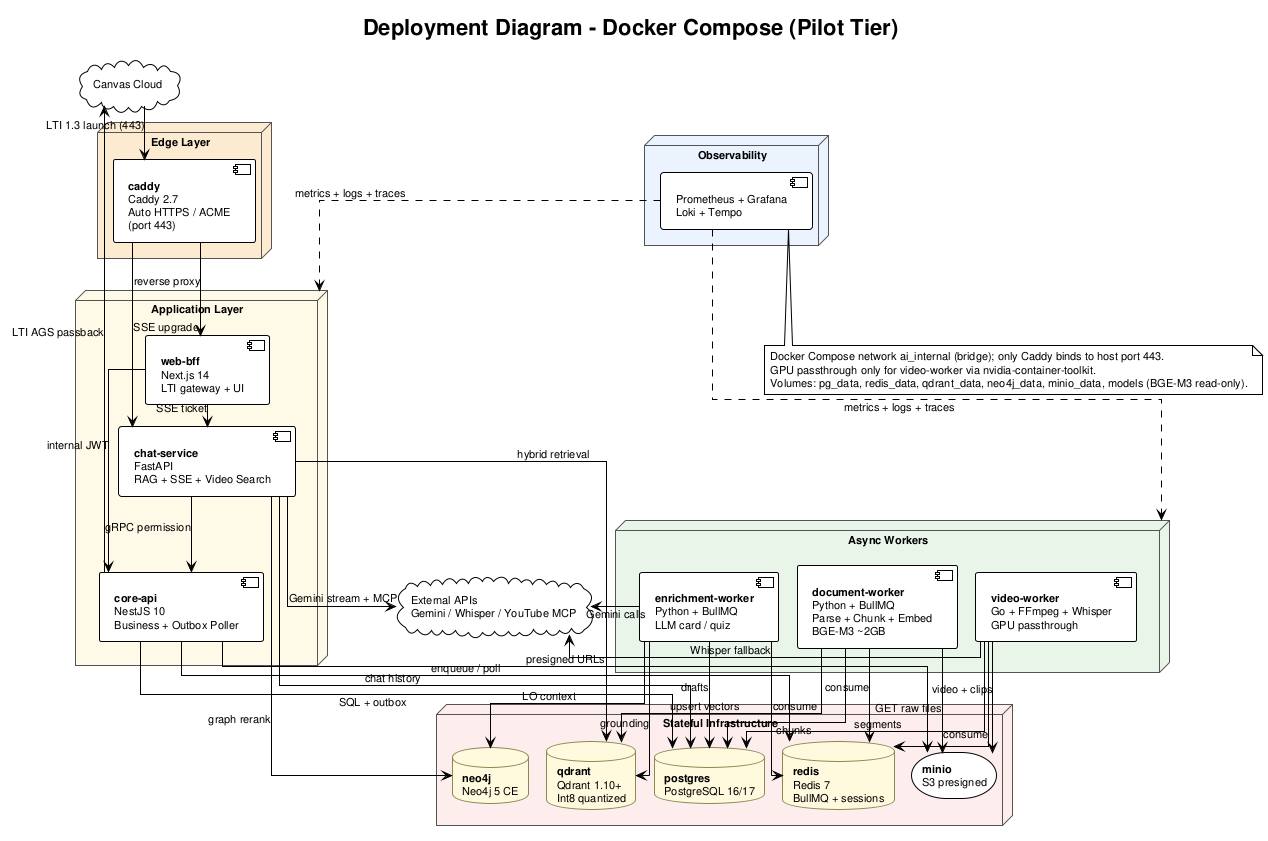
\includegraphics[width=0.95\textwidth]{diagrams/deployment_diagram.png}
    \caption{Deployment diagram of the pilot system.}
    \label{fig:deployment-implementation-lvtn}
\end{figure}

\subsection{\texttt{web-bff} (Next.js)}

The frontend and Backend-for-Frontend are implemented with Next.js 14
and App Router. The component has three main roles:

\begin{itemize}
    \item Server-side rendering for instructors (\texttt{/manage/*})
          and students (\texttt{/learn/*}).
    \item Receiving LTI launches and issuing sessions through
          \texttt{HttpOnly}, \texttt{SameSite=None}, \texttt{Secure}
          cookies, which are required because the tool runs inside a
          Canvas iframe.
    \item Proxying requests from the UI to \texttt{core-api} and
          \texttt{chat-service}, with a short-lived BFF-to-Core JWT.
\end{itemize}

Main route structure (App Router):

\begin{itemize}
    \item \texttt{app/lti/login/route.ts}: OIDC login initialization,
          storing \texttt{state} + \texttt{nonce} in Redis (TTL 5
          minutes), then redirecting to the Canvas authorize endpoint.
    \item \texttt{app/lti/launch/route.ts}: receives form POST, verifies
          the \texttt{id\_token} JWT through Canvas JWKS, maps the user,
          sets the session cookie, and redirects by role.
    \item \texttt{app/manage/review/page.tsx}: review inbox, list of
          draft cards/quizzes, approve/reject/edit actions.
    \item \texttt{app/manage/documents/page.tsx}: upload and document
          list.
    \item \texttt{app/learn/lessons/[id]/page.tsx}: card view and
          navigation.
    \item \texttt{app/learn/lessons/[id]/quiz/page.tsx}: quiz-taking
          screen.
    \item \texttt{app/learn/chat/page.tsx}: AI Tutor chatbot.
    \item \texttt{app/api/sse-chat/route.ts}: proxies SSE from
          \texttt{chat-service} back to the browser without buffering.
\end{itemize}

The LTI session is stored server-side (Redis) instead of only in a
cookie to reduce the risk of exposing sensitive claims and to support
immediate invalidation on logout. The frontend does not make business
authorization decisions by itself; every authorization decision is
delegated to \texttt{core-api} through JWT.

\subsection{\texttt{core-api} (NestJS)}

\texttt{core-api} is implemented with NestJS 10 and the Fastify adapter
to reduce overhead compared with Express. It acts as the business center:

\begin{itemize}
    \item Metadata management: \texttt{documents}, \texttt{videos},
          \texttt{lesson\_cards}, \texttt{quiz\_items}, \texttt{courses}.
    \item Authorization: verifies \texttt{Instructor}/\texttt{Learner}
          roles in the course context extracted from JWT.
    \item Review/Publish: state machine for cards/quizzes, audit-log
          writing.
    \item Job orchestration: publishes events to BullMQ, through HTTP
          \texttt{BullMQ Pro} or directly through a Redis client.
    \item Hosts the Outbox Poller daemon running in-process.
\end{itemize}

Module structure (NestJS): each bounded context has one module
(\texttt{CourseModule}, \texttt{DocumentModule}, \texttt{ContentModule},
\texttt{ReviewModule}, \texttt{AnalyticsModule}, \texttt{OutboxModule}),
and each module contains \texttt{*.controller.ts}, \texttt{*.service.ts},
\texttt{*.repository.ts}, and \texttt{*.dto.ts}.

ORM: Prisma is used for queries and migrations. It is chosen instead of
TypeORM because it generates a type-safe client, uses a schema as a
single source of truth, and provides a good migration CLI for the team.

\subsection{\texttt{chat-service} (FastAPI)}

\texttt{chat-service} is implemented with FastAPI 0.110+ and Uvicorn
(2 worker processes, without Gunicorn so the async event loop remains
simple). It exposes two main endpoints:

\begin{itemize}
    \item \texttt{POST /chat/ticket}: issues a Single-Use Ticket for
          the client to open SSE. It verifies the BFF-to-Core JWT,
          generates a ticket UUID, and stores it in Redis with TTL 60s.
    \item \texttt{GET /chat/stream?ticket=...\&q=...}: verifies the
          ticket, consumes it so it can only be used once, executes RAG,
          and streams tokens through \texttt{StreamingResponse} with MIME
          type \texttt{text/event-stream}.
\end{itemize}

The internal pipeline in \texttt{stream}:

\begin{enumerate}
    \item Generate dense+sparse embeddings with BGE-M3.
    \item Search Qdrant hybrid with a hard \texttt{course\_id} filter.
    \item Apply Reciprocal Rank Fusion.
    \item Query Neo4j for LO context (graph-aware reranking).
    \item Build the prompt and call Gemini Pro streaming.
    \item Yield each token with citation markers.
    \item Persist \texttt{chat\_messages} to PostgreSQL after streaming
          completes.
\end{enumerate}

\subsection{\texttt{document-worker}}

\texttt{document-worker} is implemented with Python 3.11 and the BullMQ
Python client (\texttt{bullmq-python}). The container has three main
roles in the same process:

\begin{itemize}
    \item \textbf{Document processing consumer:} downloads files from
          MinIO, parses them (PyMuPDF for text layers, Docling for OCR),
          chunks by headings, embeds with BGE-M3, and upserts to Qdrant.
    \item \textbf{Graph sync consumer:} consumes Outbox events from
          PostgreSQL, relayed by \texttt{core-api}, to create nodes and
          relationships in Neo4j through Cypher \texttt{MERGE}.
    \item \textbf{Curriculum ingestion consumer:} consumes
          \texttt{CurriculumIngestionRequested}, uses Gemini Flash to
          parse the syllabus PDF into Course/Chapter/LO/Assessment.
\end{itemize}

\texttt{BGE-M3} is loaded lazily on the first job, reducing 10--15
seconds of startup time if the container restarts repeatedly, and then
kept in RAM for all following jobs. Each job uses the Hexagonal use case
\texttt{ProcessDocumentUseCase.execute(document\_id)} to isolate logic
from the BullMQ framework, which allows unit tests to run without
spinning up Redis.

\subsection{\texttt{enrichment-worker}}

\texttt{enrichment-worker} consumes the
\texttt{ContentGenerationRequested} event (type=card or quiz), groups
chunks by level-2 heading or by LO, builds a prompt with strict JSON
schema, calls Gemini Pro/Flash, validates the output, and persists the
artifact with status \texttt{GENERATED\_DRAFT}.

This worker is I/O-bound: each LLM call can take 5--30 seconds. It is
configured with \texttt{concurrency=10} (10 concurrent jobs), instead
of 1 as in CPU-bound workers. When Gemini returns HTTP 429 (rate limit),
BullMQ uses exponential backoff and retries 3 times ($1s \to 2s \to
4s$); after that, it switches to a fallback model (Gemini Flash instead
of Pro) and retries one more time.

\subsection{\texttt{video-worker} (Go)}

\texttt{video-worker} is implemented with Go 1.22+ instead of Python
to: (i) avoid the GIL when orchestrating parallel FFmpeg subprocesses
through goroutines, (ii) build a small static binary ($\approx$ 20MB)
instead of a Python image ($\approx$ 1GB), and (iii) handle large
streams more reliably with Go's \texttt{io.Pipe}.

The pipeline for each job:

\begin{enumerate}
    \item Download the video from MinIO through a presigned URL stream
          without loading the whole file into RAM.
    \item Run \texttt{ffmpeg -i input.mp4 -vn -acodec pcm\_s16le -ar
          16000} to extract 16kHz mono audio for Whisper.
    \item Call Whisper through a \texttt{whisper.cpp} binding (local) or
          HTTP API (fallback). The output is a word-timestamped
          transcript.
    \item Detect segment boundaries using silence $\geq 1.5s$ plus
          topic shift (cosine similarity between segment embeddings
          $< 0.7$).
    \item Cut 30--90 second clips with \texttt{ffmpeg -ss ... -t ... -c
          copy} without re-encoding.
    \item Upload clips back to MinIO, insert
          \texttt{video\_segments}/\texttt{transcript\_segments} into
          PostgreSQL.
    \item Publish \texttt{TranscriptReady} for \texttt{document-worker}
          to embed.
\end{enumerate}

Because processing a 60-minute video may exceed 30 minutes, which is
the default stalled-job threshold in BullMQ, the worker calls
\texttt{job.updateProgress()} every 10 seconds to confirm progress.

\section{Hexagonal Port Adapter Implementation}
\label{sec:adapter-impl}

\begin{figure}[H]
    \centering
    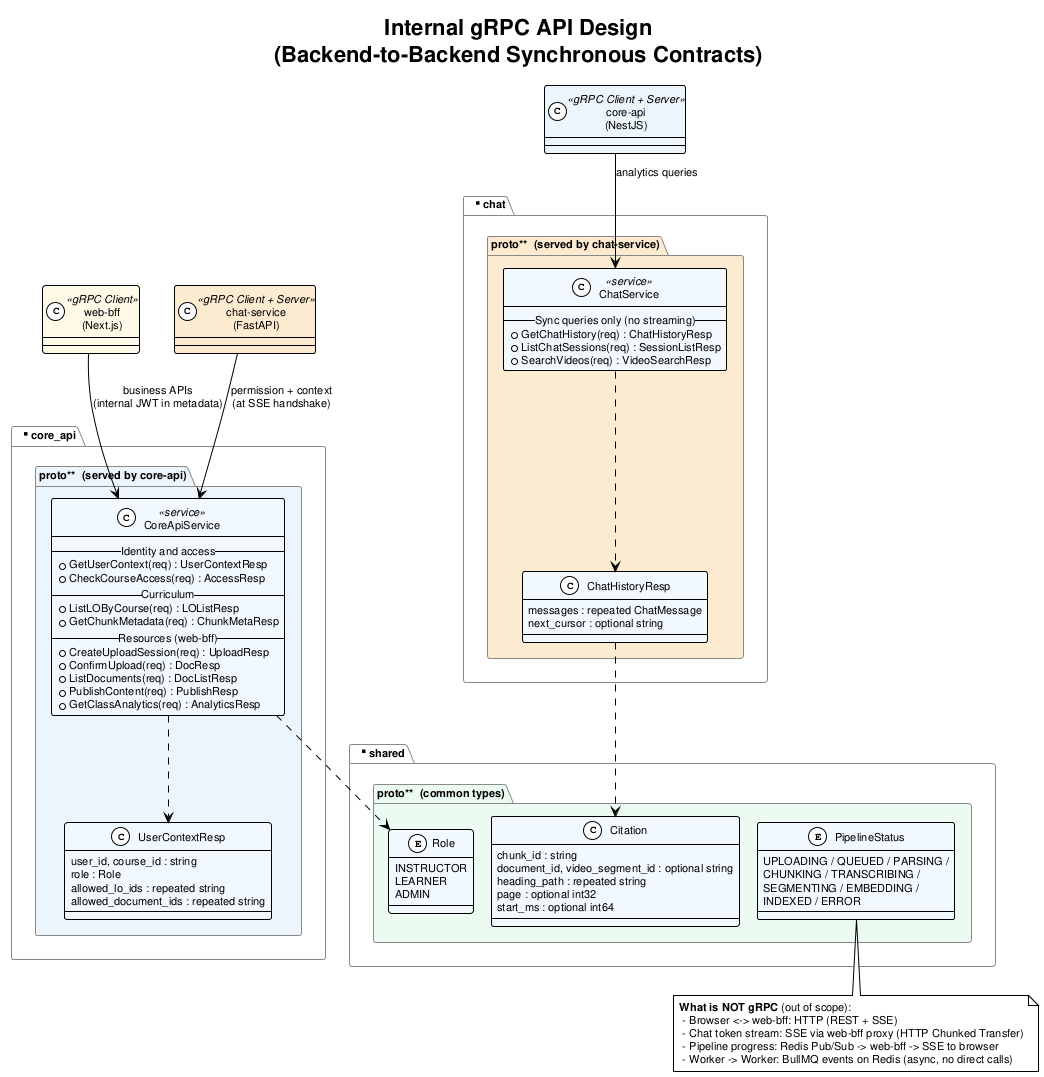
\includegraphics[width=0.95\textwidth]{diagrams/grpc_service_design.png}
    \caption{Relationship between Ports (\textit{abstract}) and Adapters
        (\textit{concrete}) in the stack.}
    \label{fig:grpc-implementation-lvtn}
\end{figure}

The seven main Ports in the Domain layer are implemented through
Adapters that can be selected by environment, as shown in the provider
matrix in Table~\ref{tab:provider-matrix}. Store adapters
(\texttt{IMetadataStore}, \texttt{IVectorStore}, \texttt{IGraphStore},
\texttt{IObjectStorage}) are fixed to the selected infrastructure, while
provider adapters (\texttt{ILLMClient}, \texttt{IEmbeddingModel},
\texttt{ISpeechToText}) support multiple backends so development can run
the full pipeline without a GPU. All adapters are wired into Use Cases
through Dependency Injection at bootstrap and do not change at runtime.

\begin{longtable}{|p{3.3cm}|p{4cm}|p{6.2cm}|}
\caption{Seven main Ports and corresponding adapter libraries.}
\label{tab:adapter-overview} \\
\hline
\textbf{Port} & \textbf{Main adapter} & \textbf{Implementation notes} \\
\hline
\endfirsthead
\hline
\textbf{Port} & \textbf{Main adapter} & \textbf{Implementation notes} \\
\hline
\endhead

\texttt{IMetadataStore}
    & Prisma (TS) / SQLAlchemy 2.0 async (Python)
    & Pool 20 for core-api, 10 for each worker. \\
\hline
\texttt{IVectorStore}
    & \texttt{qdrant-client} 1.10+
    & Hybrid \texttt{query\_points} with dense+sparse
      \texttt{prefetch} and \texttt{FusionQuery("rrf")}; hard
      \texttt{course\_id} filter. \\
\hline
\texttt{IGraphStore}
    & Neo4j Python driver 5.x
    & Separate Read/Write sessions; every mutation uses Cypher
      \texttt{MERGE} to guarantee idempotency. \\
\hline
\texttt{IObjectStorage}
    & \texttt{minio-py} / \texttt{minio-go}
    & Presigned upload URL + stream download for workers. \\
\hline
\texttt{ILLMClient}
    & \texttt{google-genai} / \texttt{openai}
    & Switch through \texttt{LLM\_PROVIDER}; strict JSON schema maps to
      \texttt{response\_schema} (Gemini) or \texttt{response\_format}
      (OpenAI). \\
\hline
\texttt{IEmbeddingModel}
    & \texttt{FlagEmbedding} (BGE-M3 local) / OpenAI
      \texttt{text-embedding-}\allowbreak\texttt{3-large}
    & Switch through \texttt{EMBEDDING\_PROVIDER}; OpenAI only provides
      dense vectors, so RRF falls back to dense-only in dev. \\
\hline
\texttt{ISpeechToText}
    & \texttt{whisper.cpp} (local) / OpenAI Whisper API /
      AssemblyAI
    & Switch through \texttt{STT\_PROVIDER}; local mode requires
      4--8GB VRAM. \\
\hline
\end{longtable}

\section{Asynchronous Infrastructure and Outbox}
\label{sec:async-impl}

\subsection{BullMQ Queue Layout}

The four main queues in Redis are:

\begin{longtable}{|p{4cm}|p{2.5cm}|p{7cm}|}
\caption{Four main BullMQ queues.}
\label{tab:bullmq-queues} \\
\hline
\textbf{Queue} & \textbf{Consumer} & \textbf{Job type} \\
\hline
\endfirsthead
\hline
\textbf{Queue} & \textbf{Consumer} & \textbf{Job type} \\
\hline
\endhead

\texttt{document-}\allowbreak\texttt{processing-q}
    & \texttt{document-}\allowbreak\texttt{worker}
    & Parse + chunk + embed PDF; reindex; graph sync. \\
\hline
\texttt{video-}\allowbreak\texttt{processing-q}
    & \texttt{video-}\allowbreak\texttt{worker}
    & Extract audio + Whisper + segment + clip. \\
\hline
\texttt{content-}\allowbreak\texttt{enrichment-q}
    & \texttt{enrichment-}\allowbreak\texttt{worker}
    & Generate cards; generate quizzes; curriculum extraction. \\
\hline
\texttt{outbox-}\allowbreak\texttt{relay-q}
    & \texttt{document-}\allowbreak\texttt{worker} (graph) or
    \texttt{core-api} fanout
    & Relay outbox events to Neo4j or downstream services. \\
\hline
\end{longtable}

\subsection{Outbox Poller Daemon}

The Outbox Poller runs in-process inside \texttt{core-api} (NestJS
module \texttt{OutboxModule}) with cron \texttt{*/5 * * * * *} (every
5 seconds):

\begin{enumerate}
    \item Query \texttt{outbox\_events WHERE status='PENDING' ORDER BY
          occurred\_at LIMIT 100 FOR UPDATE SKIP LOCKED}.
    \item Convert each event into a BullMQ job with
          \texttt{jobId = outbox\_id} (idempotent).
    \item When BullMQ \texttt{add()} succeeds, update
          \texttt{status='PROCESSED'} and write
          \texttt{processed\_at}.
    \item If \texttt{add()} fails, keep \texttt{status='PENDING'},
          increment \texttt{retry\_count}, and after 5 failures set
          \texttt{status='FAILED'} and write \texttt{last\_error}.
\end{enumerate}

\subsection{Retry Policy and Dead Letter Queue}

Each BullMQ queue is configured as follows:

\begin{itemize}
    \item \texttt{attempts=3}, \texttt{backoff={type:'exponential',
          delay:1000}} $\to$ retry after 1s, 2s, and 4s.
    \item After exceeding \texttt{attempts}, the job is moved to
          BullMQ's \texttt{failed} list. A queue dashboard
          (\texttt{bull-board} or Arena) allows an engineer to requeue
          jobs manually.
    \item Jobs that fail because of corrupt files are tagged
          \texttt{discardOnError=true} so the system does not waste LLM
          tokens on retries.
\end{itemize}

\subsection{Consumer Idempotency}

\begin{itemize}
    \item Chunks use UUIDv7 as primary keys; \texttt{INSERT ... ON
          CONFLICT (chunk\_id) DO UPDATE} is used for upsert.
    \item Qdrant upserts by \texttt{chunk\_id}, making the operation
          idempotent.
    \item Neo4j uses \texttt{MERGE} instead of \texttt{CREATE}.
    \item BullMQ \texttt{jobId} is uniquely bound to
          \texttt{outbox\_id}, so the same event cannot be enqueued
          twice.
\end{itemize}

\section{Canvas LMS Integration through LTI 1.3}
\label{sec:lti-impl}

\subsection{Canvas Developer Key Configuration}

The procedure for registering the Tool in Canvas (Cloud sandbox for
dev/pilot) is:

\begin{enumerate}
    \item Create a Developer Key of type \textit{LTI Key} in Canvas
          Admin.
    \item Configure \texttt{Target Link URI} =
          \texttt{https://lvtn-ai.example/lti/launch},
          \texttt{OIDC Initiation URL} =
          \texttt{https://lvtn-ai.example/lti/login},
          \texttt{JWKS URL} =
          \texttt{https://lvtn-ai.example/.well-known/jwks.json}.
    \item Enable scopes: \texttt{lineitem.readonly}, \texttt{lineitem},
          \texttt{score} (for AGS), \texttt{result.readonly},
          \texttt{names\_and\_roles} (for NRPS).
    \item Get \texttt{Client ID} and \texttt{Deployment ID} $\to$ store
          them in the \texttt{web-bff} environment.
\end{enumerate}

\subsection{OIDC Login and Launch Endpoints}

Handler structure in \texttt{web-bff}:

\begin{itemize}
    \item \texttt{/lti/login}: receives \texttt{iss},
          \texttt{login\_hint}, \texttt{client\_id},
          \texttt{target\_link\_uri}; generates cryptographically random
          \texttt{state} and \texttt{nonce}; stores them in Redis with
          TTL 5 minutes; redirects 302 to
          \texttt{{iss}/api/lti/authorize\_redirect}.
    \item \texttt{/lti/launch}: receives a form POST containing
          \texttt{id\_token} (JWT) and \texttt{state}; verifies that
          state matches Redis, verifies that nonce has not been used,
          verifies the JWT signature through Canvas JWKS (cached for
          24h), verifies \texttt{aud}, \texttt{exp}, \texttt{iss};
          extracts \texttt{sub} (LMS user ID), \texttt{context.id}
          (course ID), and \texttt{roles}; upserts
          \texttt{lms\_user\_mappings} through \texttt{core-api}; sets
          the session cookie.
\end{itemize}

\subsection{BFF-to-Core JWT Signing}

\texttt{web-bff} has an Ed25519 key pair generated at bootstrap. Each
request proxied to \texttt{core-api} or \texttt{chat-service} carries a
new JWT with TTL 60s and these claims:

\begin{itemize}
    \item \texttt{sub}: internal user ID (UUID).
    \item \texttt{course\_id}: the currently launched course (omitted for
          admin tokens).
    \item \texttt{roles}: one of \texttt{Instructor},
          \texttt{Learner}, or \texttt{Administrator}. Course-context
          roles (instructor/learner/ta/observer) are resolved against
          \texttt{course\_memberships} on the server side after JWT
          verification.
    \item \texttt{scope}: \texttt{course} (default) or \texttt{admin}.
          Admin-scope tokens are minted only for users with
          \texttt{lms\_user\_mappings.role = administrator} and authorize
          only the \texttt{/admin/*} surface; they cannot read or write
          course content.
    \item \texttt{jti}: random UUID to prevent replay.
    \item \texttt{exp}, \texttt{iat}.
\end{itemize}

\texttt{core-api} and \texttt{chat-service} verify the JWT using BFF's
public key, loaded from a ConfigMap or environment variable. The public
key can be rotated when needed.

\subsection{Assignment and Grade Services (AGS)}

After a student submits a quiz, \texttt{core-api} grades it and calls
AGS passback:

\begin{enumerate}
    \item Request an OAuth 2.0 access token from Canvas
          (\texttt{client\_credentials} grant with a private-key JWT
          assertion).
    \item POST to \texttt{lineitems/{id}/scores} with payload
          \texttt{{userId, scoreGiven, scoreMaximum, activityProgress,
          gradingProgress}}.
    \item Cache the token for 50 minutes (Canvas token TTL is 1 hour).
\end{enumerate}

\subsection{Deep Linking (for Instructor Placement)}

Instructors can select a specific lesson and attach it to a Canvas
activity through Deep Linking 2.0:

\begin{itemize}
    \item Canvas redirects to \texttt{/lti/deep-link-select} with
          \texttt{deep\_link\_return\_url}.
    \item The instructor selects a lesson from the UI. BFF generates an
          \texttt{LtiResourceLinkRequest} JWT and POSTs it back to
          \texttt{deep\_link\_return\_url}.
    \item Canvas creates an activity with \texttt{custom.lesson\_id}
          embedded in the next launch context.
\end{itemize}

\section{Docker Compose Packaging}
\label{sec:docker-compose}

\subsection{Compose File Organization}

The stack is configured through one base file and two overrides:
\texttt{docker-compose.yml} (pilot base), \texttt{docker-compose.dev.yml}
(mount source code, expose DB ports to the host), and
\texttt{docker-compose.gpu.yml} (enable GPU for \texttt{video-worker}
and \texttt{document-worker}). Commands for each configuration:

\begin{lstlisting}[language=bash, caption={Running the stack by configuration.}]
# Pilot without GPU
docker compose -f infra/docker-compose.yml up -d --build

# Pilot with GPU (gpu overlay file)
docker compose -f infra/docker-compose.yml \
  -f infra/docker-compose.gpu.yml up -d --build

# Dev hot-reload (overlay file dev)
docker compose -f infra/docker-compose.yml \
  -f infra/docker-compose.dev.yml up
\end{lstlisting}

\subsection{Network and Volume}

\textbf{Network:}
\begin{itemize}
    \item \texttt{ai\_internal} (bridge): internal connection for all
          services. It is not exposed to the host in the pilot.
    \item \texttt{public} (bridge): only \texttt{caddy} binds ports 80
          and 443 to the host network.
\end{itemize}

\textbf{Volume:}
\begin{itemize}
    \item \texttt{pgdata}: PostgreSQL data; daily backup through
          \texttt{pg\_dump} cron.
    \item \texttt{minio-data}: object storage.
    \item \texttt{qdrant-storage}: vector data.
    \item \texttt{neo4j-data}: graph data.
    \item \texttt{redis-data}: AOF persistence.
    \item \texttt{models} (bind mount \texttt{./models} read-only):
          contains BGE-M3 and Whisper models, shared by
          \texttt{document-worker} and \texttt{video-worker}; avoids
          re-downloading after image rebuilds.
    \item \texttt{caddy-data}, \texttt{caddy-config}: Let's Encrypt
          certificates.
\end{itemize}

\subsection{Container Resource Limits}

Each service declares \texttt{deploy.resources.limits} according to
Table~\ref{tab:ram-allocation}. Example snippet for
\texttt{document-worker}:

\begin{lstlisting}[caption={Resource limit for \texttt{document-worker}.}]
document-worker:
  image: lvtn-ai/document-worker:${TAG}
  deploy:
    resources:
      limits:
        cpus: '2.0'
        memory: 4G
      reservations:
        memory: 3G
        devices:
          - capabilities: [gpu]
            count: 1
            driver: nvidia
  environment:
    - EMBEDDING_PROVIDER=bge-m3-local
    - LLM_PROVIDER=gemini
\end{lstlisting}

\subsection{Healthcheck and Restart Policy}

Every service has a healthcheck:

\begin{itemize}
    \item HTTP services (\texttt{web-bff}, \texttt{core-api},
          \texttt{chat-service}): \texttt{GET /health} every 30s.
    \item Workers: call \texttt{redis-cli PING} or expose a Prometheus
          metrics port with endpoint \texttt{/healthz}.
    \item Databases: use the built-in healthcheck of the image
          (\texttt{pg\_isready}, \texttt{redis-cli ping},
          \texttt{curl} to Qdrant \texttt{/healthz}).
\end{itemize}

\texttt{restart: unless-stopped} is used for every service except
one-shot containers such as the migration runner.

\section{CI/CD and Configuration Environment}
\label{sec:cicd-impl}

\subsection{GitHub Actions Workflow}

The CI/CD pipeline is split into four jobs that run in parallel when
possible:

\begin{enumerate}
    \item \textbf{Lint + type check}: \texttt{ruff} + \texttt{mypy}
          (Python), \texttt{eslint} + \texttt{tsc} (TS),
          \texttt{golangci-lint} (Go).
    \item \textbf{Unit test}: \texttt{pytest} (Python),
          \texttt{vitest} or \texttt{jest} (TS), \texttt{go test} (Go).
    \item \textbf{Integration test}: bring up testcontainers with
          docker compose (Postgres + Redis + Qdrant + MinIO) and run
          integration tests that call real RPC/HTTP paths between
          services.
    \item \textbf{Build + push image}: build a Docker image for each
          runtime with tag \texttt{$\{$ commit SHA $\}$}, then push to
          GHCR.
\end{enumerate}

Staging deployment is automatic after merge to \texttt{main}; production
deployment requires manual approval.

\subsection{Secret and Environment Variable Management}

\begin{itemize}
    \item \textbf{Dev:} \texttt{.env.local} (gitignored), containing
          dev-tier LLM API keys.
    \item \textbf{CI:} GitHub Actions Secrets, injected into jobs
          through \texttt{secrets.*}.
    \item \textbf{Pilot:} a \texttt{.env} file on the VPS host with mode
          \texttt{600}, never committed. It can later move to
          \texttt{docker secret} or HashiCorp Vault in production.
\end{itemize}

Table~\ref{tab:env-vars} groups the main environment variables into
five functional groups:

\begin{longtable}{|p{3cm}|p{10.5cm}|}
\caption{Main environment variables grouped by function.}
\label{tab:env-vars} \\
\hline
\textbf{Group} & \textbf{Variables and description} \\
\hline
\endfirsthead
\hline
\textbf{Group} & \textbf{Variables and description} \\
\hline
\endhead

Data store
    & \texttt{POSTGRES\_URL}, \texttt{REDIS\_URL}, \texttt{QDRANT\_URL},
      \texttt{NEO4J\_URI/USER/PASSWORD},
      \texttt{MINIO\_ENDPOINT/ACCESS\_KEY/SECRET\_KEY}. \\
\hline
Provider switching
    & \texttt{LLM\_PROVIDER} (\texttt{gemini}/\texttt{openai}),
      \texttt{EMBEDDING\_PROVIDER}
      (\texttt{bge-m3-local}/\texttt{openai}),
      \texttt{STT\_PROVIDER}
      (\texttt{whisper-local}/\texttt{openai}/\texttt{assemblyai}),
      \texttt{GEMINI\_API\_KEY}, \texttt{OPENAI\_API\_KEY}. \\
\hline
LTI / Canvas
    & \texttt{LTI\_CLIENT\_ID}, \texttt{LTI\_DEPLOYMENT\_ID},
      \texttt{LTI\_ISSUER}, \texttt{LTI\_JWKS\_URL}. \\
\hline
Internal JWT
    & \texttt{BFF\_JWT\_PRIVATE\_KEY}, \texttt{BFF\_JWT\_PUBLIC\_KEY}
      (Ed25519 key pair for BFF-to-Core JWT). \\
\hline
Observability
    & \texttt{OTEL\_EXPORTER\_OTLP\_ENDPOINT}, \texttt{SENTRY\_DSN}. \\
\hline
\end{longtable}

\subsection{Provider Switching by Environment}

Table~\ref{tab:provider-matrix} describes the default provider
configuration by environment tier, allowing developers without a GPU to
still run the full pipeline.

\begin{longtable}{|p{2.5cm}|p{3.5cm}|p{3.5cm}|p{3.5cm}|}
\caption{Default providers by tier.}
\label{tab:provider-matrix} \\
\hline
\textbf{Tier} & \textbf{Embedding} & \textbf{STT} & \textbf{LLM} \\
\hline
\endfirsthead
\hline
\textbf{Tier} & \textbf{Embedding} & \textbf{STT} & \textbf{LLM} \\
\hline
\endhead

\texttt{dev} & OpenAI text-embedding-3 & OpenAI Whisper API &
    Gemini Flash \\
\hline
\texttt{ci} & Mock & Mock & Mock \\
\hline
\texttt{pilot} (no GPU) & OpenAI text-embedding-3 & OpenAI Whisper API
    & Gemini Pro \\
\hline
\texttt{pilot} (with GPU) & BGE-M3 local & Whisper local &
    Gemini Pro \\
\hline
Production & BGE-M3 local & Whisper local + AssemblyAI fallback
    & Gemini Pro + OpenAI fallback \\
\hline
\end{longtable}

\section{Chapter Summary}

This chapter has presented concrete implementation decisions:

\begin{itemize}
    \item \textbf{Target environment:} Ubuntu Server 22.04 LTS for the
          pilot; dev supports macOS/Windows WSL2/Linux. Minimum pilot
          RAM ranges from 16GB (without GPU) to 32GB (with GPU); total
          container allocation is around 20GB.
    \item \textbf{Source-code structure:} pnpm + Poetry monorepo with 6
          runtime apps and shared packages; each Python worker follows a
          strict Hexagonal layout.
    \item \textbf{6 runtimes:} \texttt{web-bff} (Next.js),
          \texttt{core-api} (NestJS), \texttt{chat-service} (FastAPI),
          \texttt{document-worker} and \texttt{enrichment-worker}
          (Python), \texttt{video-worker} (Go).
    \item \textbf{Environment-switchable adapters:} embedding
          (BGE-M3/OpenAI), STT (Whisper local/OpenAI/AssemblyAI), LLM
          (Gemini/OpenAI), allowing dev to run without a GPU.
    \item \textbf{Outbox poller + BullMQ} ensure eventual consistency
          between PostgreSQL, Qdrant, Neo4j, and downstream workers.
    \item \textbf{Canvas LMS integration} through LTI 1.3 OIDC, AGS
          grade passback, and Deep Linking; BFF-to-Core Ed25519 JWT
          isolates Canvas sessions from backend services.
    \item \textbf{Docker Compose} with 3 files (base + dev override +
          GPU override) is the main packaging approach; Kubernetes is a
          future direction after the thesis defense.
    \item \textbf{CI/CD:} GitHub Actions with 4 parallel jobs (lint,
          test, integration, build); secrets are managed through env
          files with mode 600 or GitHub Actions Secrets.
\end{itemize}

The next chapter, Chapter 6, presents the methodology and evaluation
results of the system based on pilot data collected according to the
plan in Section~\ref{sec:plan-gd2} of
Chapter~\ref{chap:ket-luan-huong-phat-trien}.
